%---------------------------------------------------------------------
\section{Resultados das simula��es}

Simula��o utilizando \HI{\texttt{Matlab/Simulink}}.

\subsection{Simula��o \#1}

\bigskip%
Par�metros e condi��es iniciais  :
%
\begin{align*}
  a_p &= -2\,,  &  y_p(0) &= 5\,, & \theta(0) &= 0\,, \\
  a_m &= 1\,,   &  y_m(0) &= 0\,, & \gamma &= \HI{2, 100}\,, \\
  r &= 1\,, & a_f &= 1\,.
\end{align*}

\bigskip%
\begin{figure}[H]
  \centering
  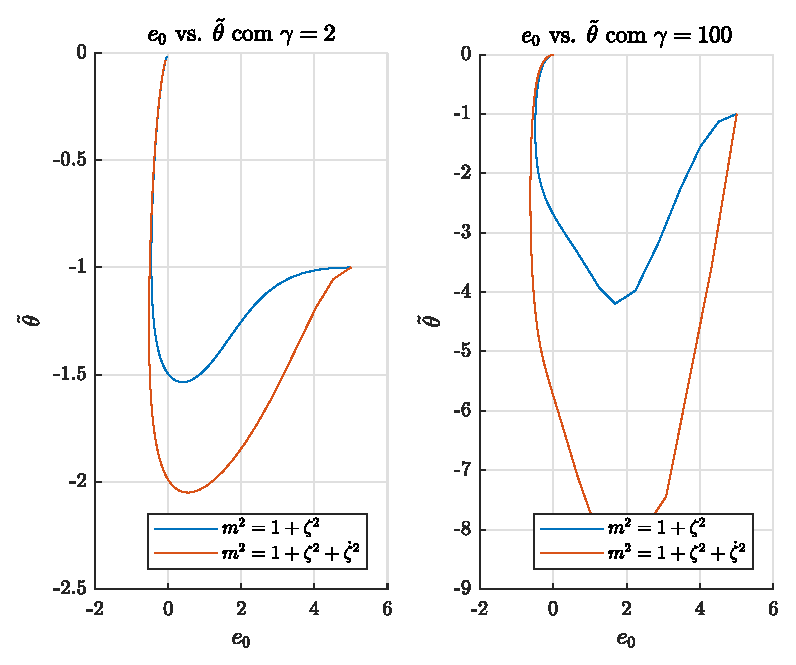
\includegraphics[width=12cm]{figs/e0_vs_deltatheta/gamma2gamma100.eps} \\[2mm]
  \caption{Diagrama $e_0 \times \tilde{\theta}$.}
\end{figure}

\begin{figure}[H]
  \centering
  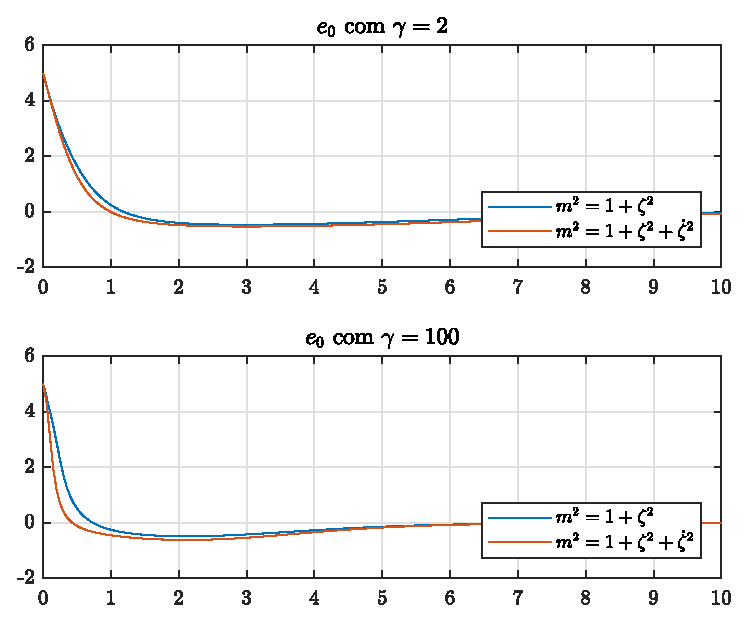
\includegraphics[width=12cm]{figs/e0/gamma2gamma100.eps}
\end{figure}

\begin{figure}[H]
  \centering
  \includegraphics[width=12cm]{figs/theta/gamma2gamma100.eps} 
\end{figure}

\begin{figure}[H]
  \centering
  \includegraphics[width=12cm]{figs/u/gamma2gamma100.eps} 
\end{figure}

\begin{figure}[H]
  \centering
  \includegraphics[width=12cm]{figs/yp/gamma2gamma100.eps} 
\end{figure}

\newpage%
%---------------------------------------------------------------------
\subsection{Simula��o \#2}
\bigskip%
Par�metros e condi��es iniciais  :
%
\begin{align*}
  a_p &= -2\,,  &  y_p(0) &= \HI{-5, 5}\,, & \theta(0) &= 0\,, \\
  a_m &= 1\,,   &  y_m(0) &= 0\,, & \gamma &= 2\,, \\
  r &= 1\,, & a_f &= 1\,.
\end{align*}

\bigskip%
\begin{figure}[H]
  \centering
  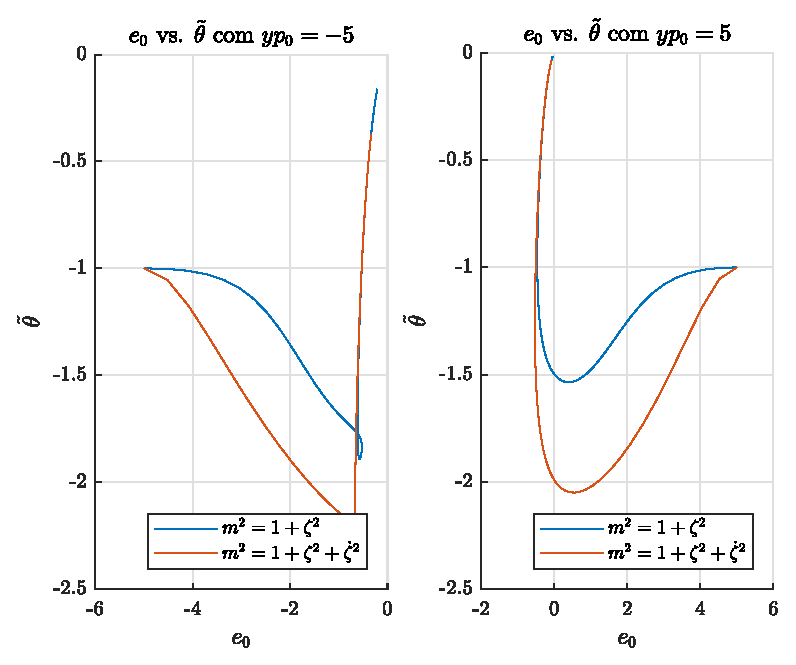
\includegraphics[width=12cm]{figs/e0_vs_deltatheta/yp0-5yp05.eps} \\[2mm]
  \caption{Diagrama $e_0 \times \tilde{\theta}$.}
\end{figure}

\begin{figure}[H]
  \centering
  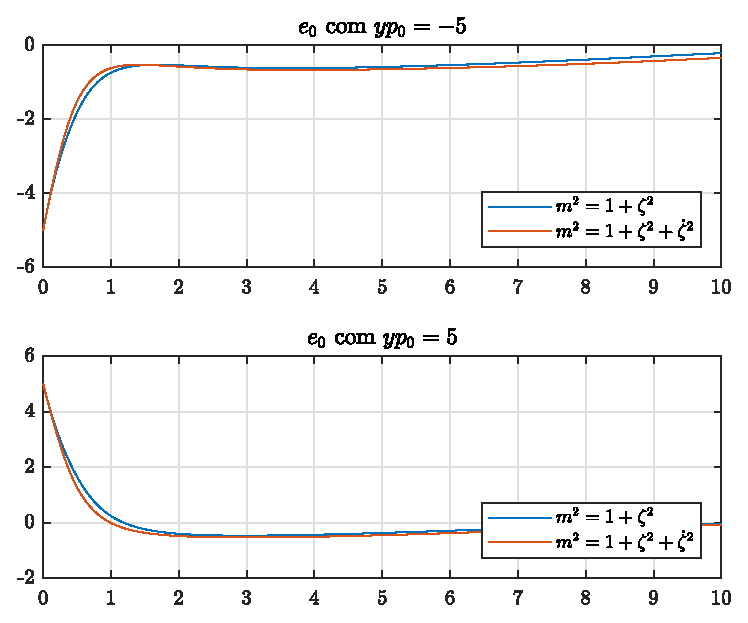
\includegraphics[width=12cm]{figs/e0/yp0-5yp05.eps}
\end{figure}

\begin{figure}[H]
  \centering
  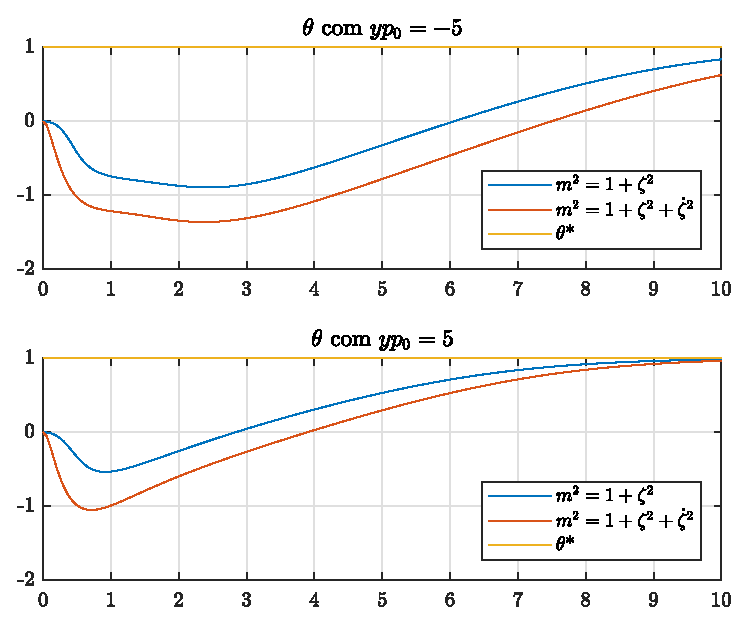
\includegraphics[width=12cm]{figs/theta/yp0-5yp05.eps} 
\end{figure}

\begin{figure}[H]
  \centering
  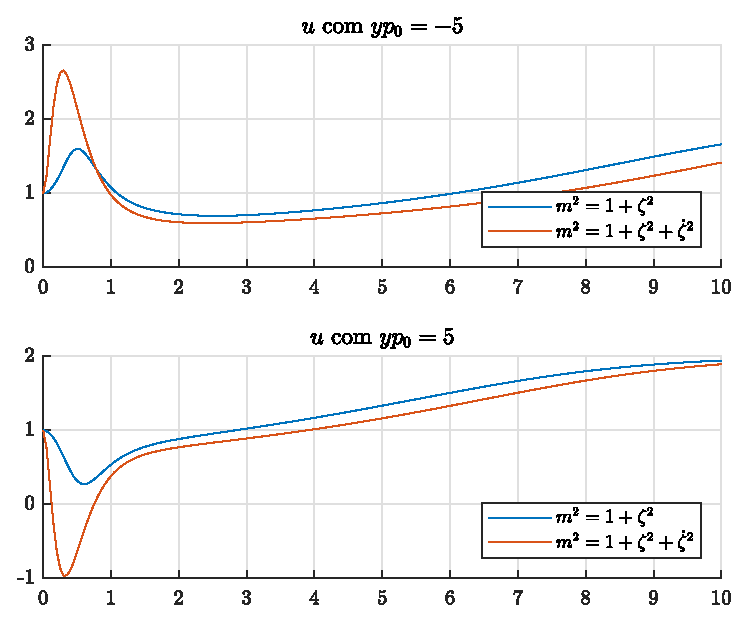
\includegraphics[width=12cm]{figs/u/yp0-5yp05.eps} 
\end{figure}

\begin{figure}[H]
  \centering
  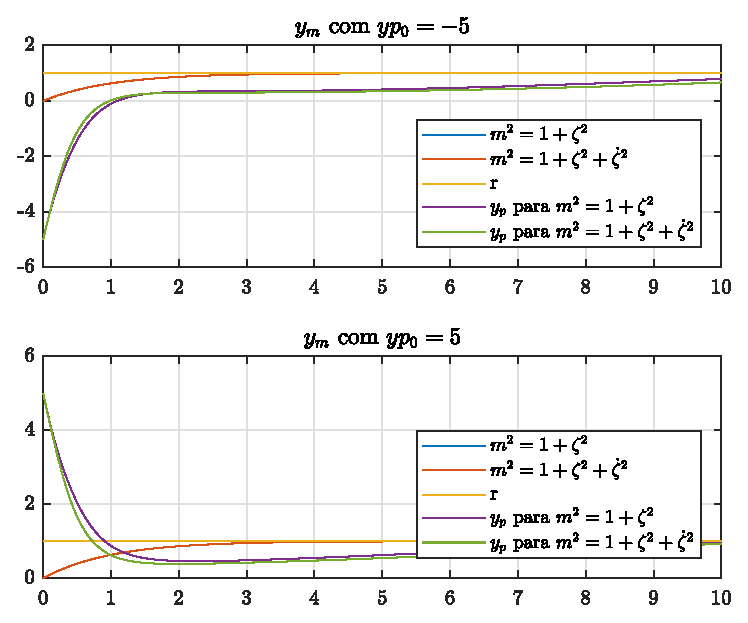
\includegraphics[width=12cm]{figs/yp/yp0-5yp05.eps} 
\end{figure}

\newpage%
%---------------------------------------------------------------------
\subsection{Simula��o \#3}

\bigskip%
Par�metros e condi��es iniciais  :
%
\begin{align*}
  a_p &= -2\,,  &  y_p(0) &= 5\,, & \theta(0) &= 0\,, \\
  a_m &= 1\,,   &  y_m(0) &= 0\,, & \gamma &= 2\,, \\
  r &= 1\,, & a_f &= \HI{1, 10}\,.
\end{align*}

\bigskip%
\begin{figure}[H]
  \centering
  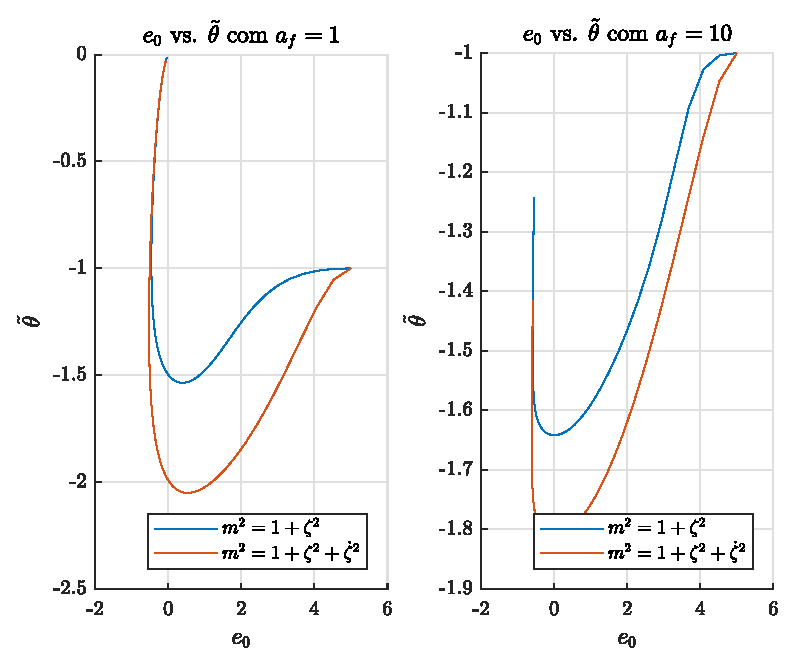
\includegraphics[width=12cm]{figs/e0_vs_deltatheta/af1af10.eps} \\[2mm]
  \caption{Diagrama $e_0 \times \tilde{\theta}$.}
\end{figure}

\begin{figure}[H]
  \centering
  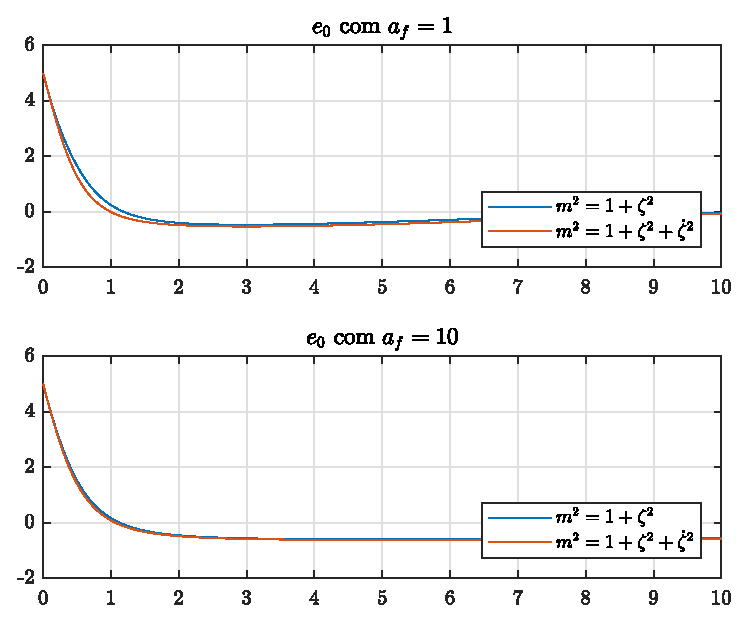
\includegraphics[width=12cm]{figs/e0/af1af10.eps}
\end{figure}

\begin{figure}[H]
  \centering
  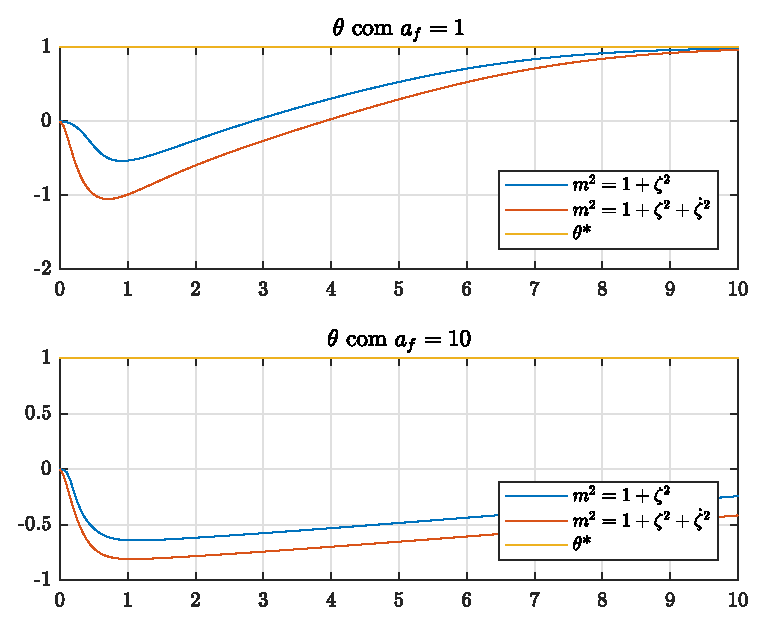
\includegraphics[width=12cm]{figs/theta/af1af10.eps} 
\end{figure}

\begin{figure}[H]
  \centering
  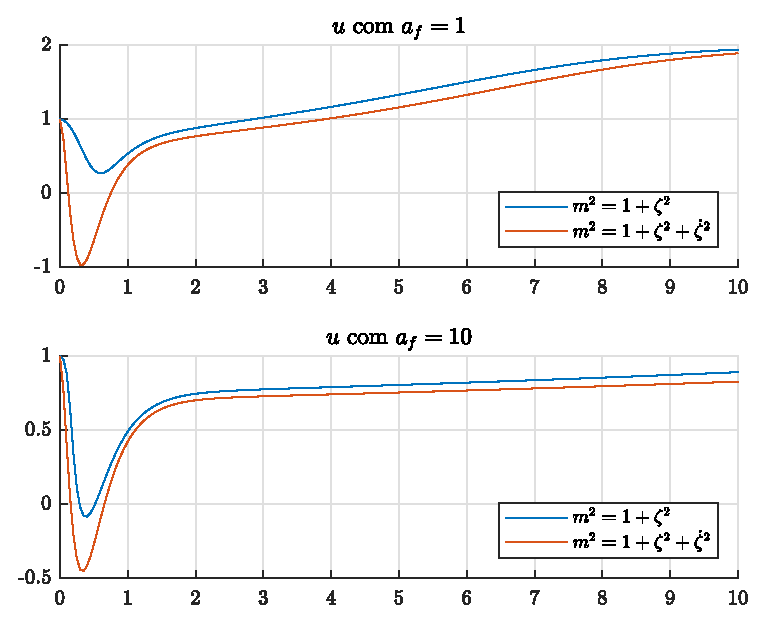
\includegraphics[width=12cm]{figs/u/af1af10.eps} 
\end{figure}

\begin{figure}[H]
  \centering
  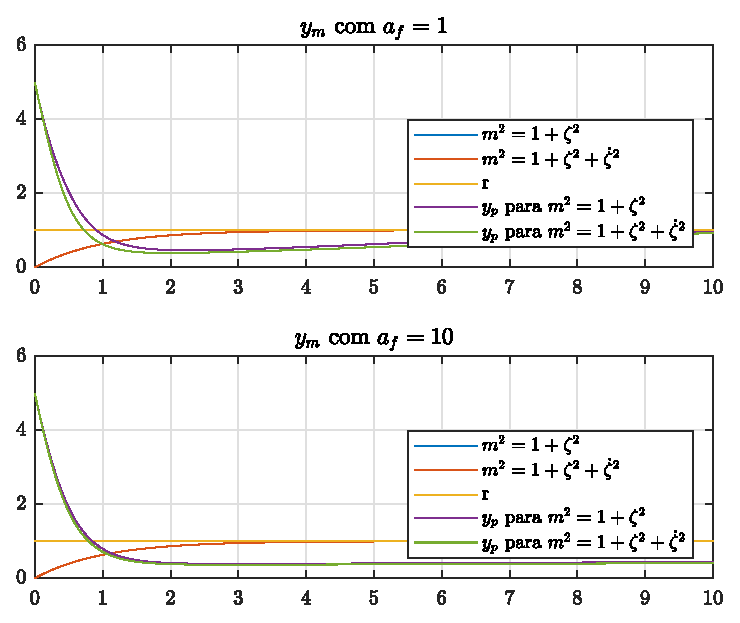
\includegraphics[width=12cm]{figs/yp/af1af10.eps} 
\end{figure}

\newpage%
%---------------------------------------------------------------------
\subsection{Simula��o \#4}
\bigskip%
Par�metros e condi��es iniciais  :
%
\begin{align*}
  a_p &= \HI{-2, -10}\,,  &  y_p(0) &= 5\,, & \theta(0) &= 0\,, \\
  a_m &= 1\,,   &  y_m(0) &= 0\,, & \gamma &= 2\,, \\
  r &= 1\,, & a_f &= 1\,.
\end{align*}

\bigskip%
\begin{figure}[H]
  \centering
  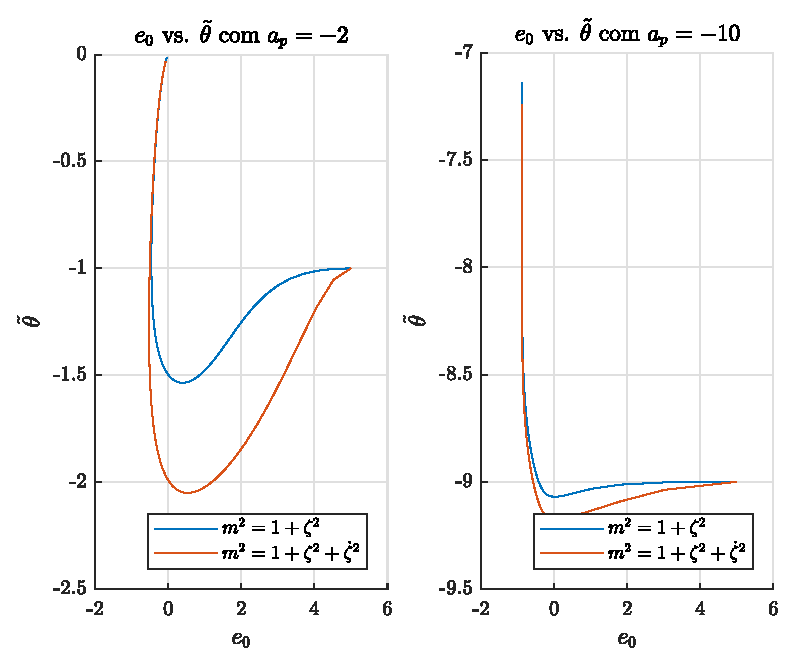
\includegraphics[width=12cm]{figs/e0_vs_deltatheta/ap-2ap-10.eps} \\[2mm]
  \caption{Diagrama $e_0 \times \tilde{\theta}$.}
\end{figure}

\begin{figure}[H]
  \centering
  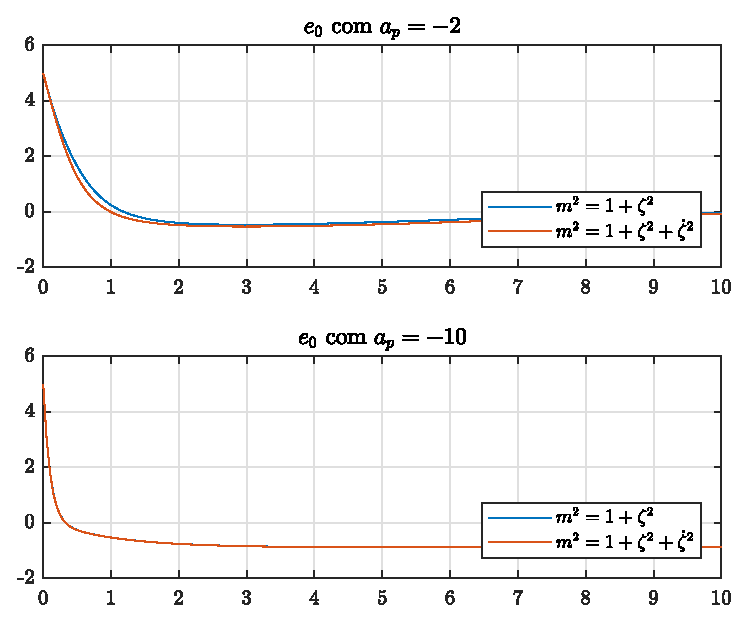
\includegraphics[width=12cm]{figs/e0/ap-2ap-10.eps}
\end{figure}
 
\begin{figure}[H]
  \centering
  \includegraphics[width=12cm]{figs/theta/ap-2ap-10.eps} 
\end{figure}

\begin{figure}[H]
  \centering
  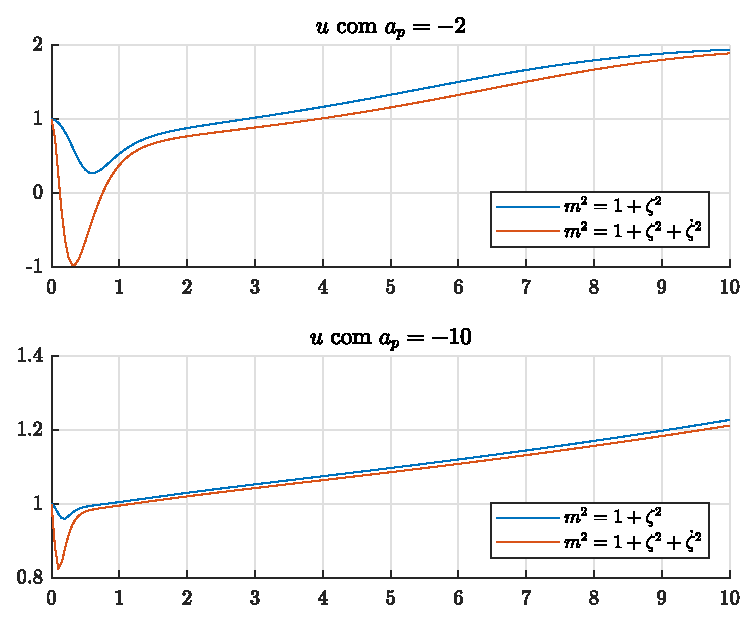
\includegraphics[width=12cm]{figs/u/ap-2ap-10.eps} 
\end{figure}

\begin{figure}[H]
  \centering
  \includegraphics[width=12cm]{figs/yp/ap-2ap-10.eps} 
\end{figure}

\newpage%
%---------------------------------------------------------------------
\subsection{Simula��o \#5}

\bigskip%
Par�metros e condi��es iniciais  :
%
\begin{align*}
  a_p &= -2\,,  &  y_p(0) &= 5\,, & \theta(0) &= 0\,, \\
  a_m &= \HI{1, 10}\,,   &  y_m(0) &= 0\,, & \gamma &= 2\,, \\
  r &= 1\,, & a_f &= 1\,.
\end{align*}

\bigskip%
\begin{figure}[H]
  \centering
  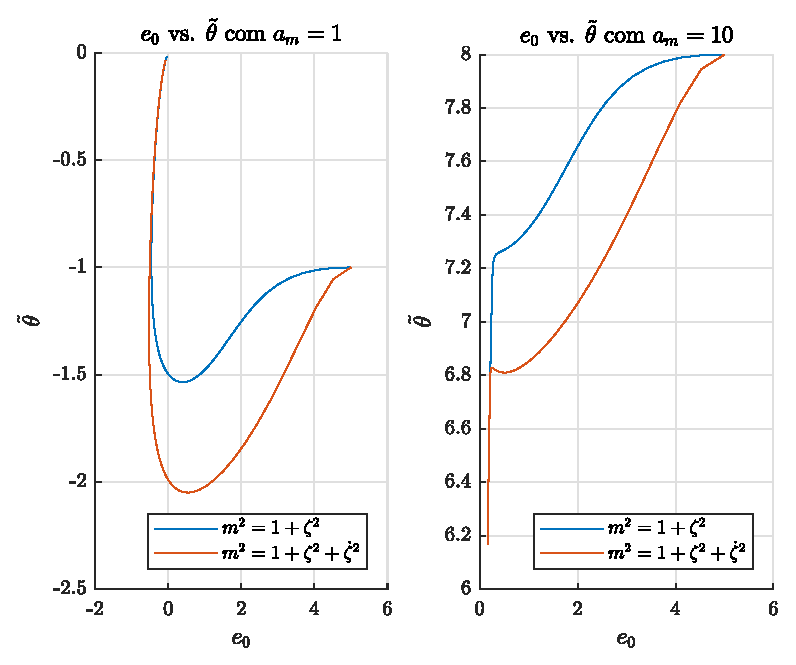
\includegraphics[width=12cm]{figs/e0_vs_deltatheta/am1am10.eps} \\[2mm]
  \caption{Diagrama $e_0 \times \tilde{\theta}$.}
\end{figure}

\begin{figure}[H]
  \centering
  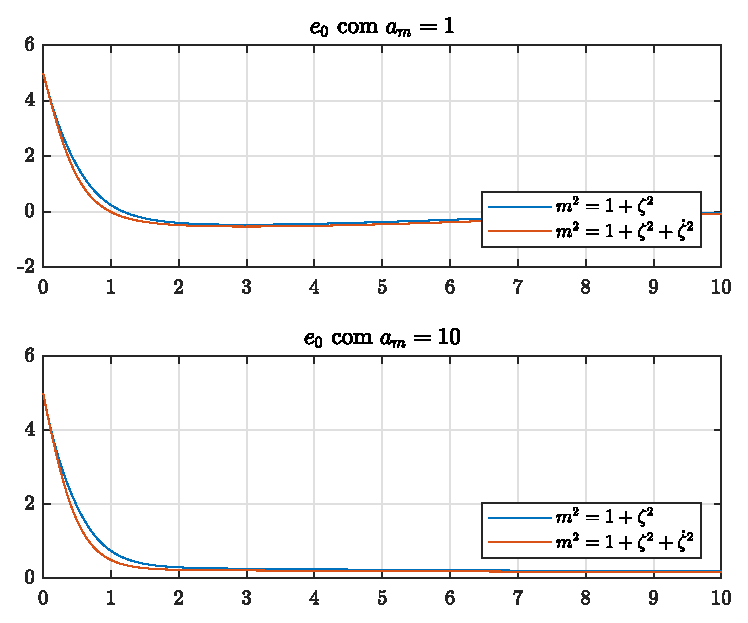
\includegraphics[width=12cm]{figs/e0/am1am10.eps}
\end{figure}

\begin{figure}[H]
  \centering
  \includegraphics[width=12cm]{figs/theta/am1am10.eps} 
\end{figure}

\begin{figure}[H]
  \centering
  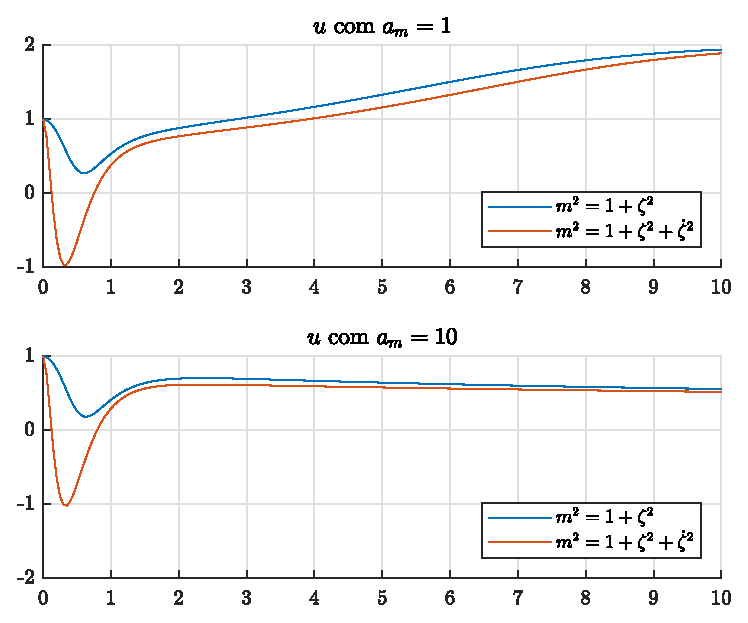
\includegraphics[width=12cm]{figs/u/am1am10.eps} 
\end{figure}

\begin{figure}[H]
  \centering
  \includegraphics[width=12cm]{figs/yp/am1am10.eps} 
\end{figure}

\newpage%
%---------------------------------------------------------------------